% Effect of the per-cell UFCS shunt on the commutation loop of the Rev B leg (fast loop-only Q3D).
% Numbers: scripts/shunt_loop_report.py -> loop_numbers.tex, loop_table.tex, figs/loop_per_cell.pdf, figs/loop_paths.pdf
\documentclass[11pt,a4paper]{article}
\usepackage[margin=22mm]{geometry}
\usepackage{booktabs,graphicx,siunitx,amsmath,caption,subcaption,hyperref,float}
% generated by scripts/shunt_loop_report.py
\newcommand{\Lbase}{0.81}
\newcommand{\Lbasezero}{0.69}
\newcommand{\Ltoponly}{0.020}
\newcommand{\Vbase}{99}
\newcommand{\Dibase}{19}
\newcommand{\Lasym}{0.12}
\newcommand{\Lvip}{0.76}
\newcommand{\Vvip}{98}
\newcommand{\Divip}{20}
\newcommand{\Lnotch}{0.73}
\newcommand{\Vnotch}{97}
\newcommand{\Dinotch}{21}
\newcommand{\Lnoshunt}{0.49}
\newcommand{\Vnoshunt}{90}
\newcommand{\Dinoshunt}{31}
\newcommand{\Lcopper}{0.20}

\title{Effect of the current shunt on the commutation loop\\\large SPB GaN leg, Rev B (4\,$\times$ EPC2361 per switch)}
\author{Enes Ayaz, KTH}
\date{October 2026}
\begin{document}
\maketitle

\section{Question}
The Rev A design reported a commutation loop of \SI{0.374}{nH} per cell. The routed Rev B leg board, with a PMK
UFCS-R001 coaxial shunt (\SI{1}{m\ohm}, \SI{120}{pH}) in the low-side source of every cell, gives \Lbase\,nH per cell
on average. This note separates the contributions and quantifies layout options for the shunt path.

\section{Model}
Fast loop-only Q3D model (\texttt{simulation/bb\_q3d/run\_bb\_q3d\_loop.cmd}): the routed copper of the board is cropped
to the band from the bypass capacitors to the shunts ($y=-4.6\ldots\SI{20.6}{mm}$), all four layers, with the transistor
stripes, both bypass rows and the shunt pads as terminals; the DC bank and the DC/AC terminals carry the
switching-frequency ripple, not the edge, and are left out. Loop as in Rev A: high-side FET of the cell shorted, bypass
groups as their ESL, the shunt as \SI{120}{pH} between its pads, \SI{1}{A} through the low-side FET of all four cells,
$L=\operatorname{Im}(V_\mathrm{LS})/\omega$ at \SI{100}{MHz}. One run takes about 45 minutes (full board: more than two
hours). Variants are generated by \texttt{SHUNT\_VARIANT} in \texttt{scripts/make\_kicad\_bb\_revb.py}.

\section{Three separate effects}
\begin{figure}[H]
\centering
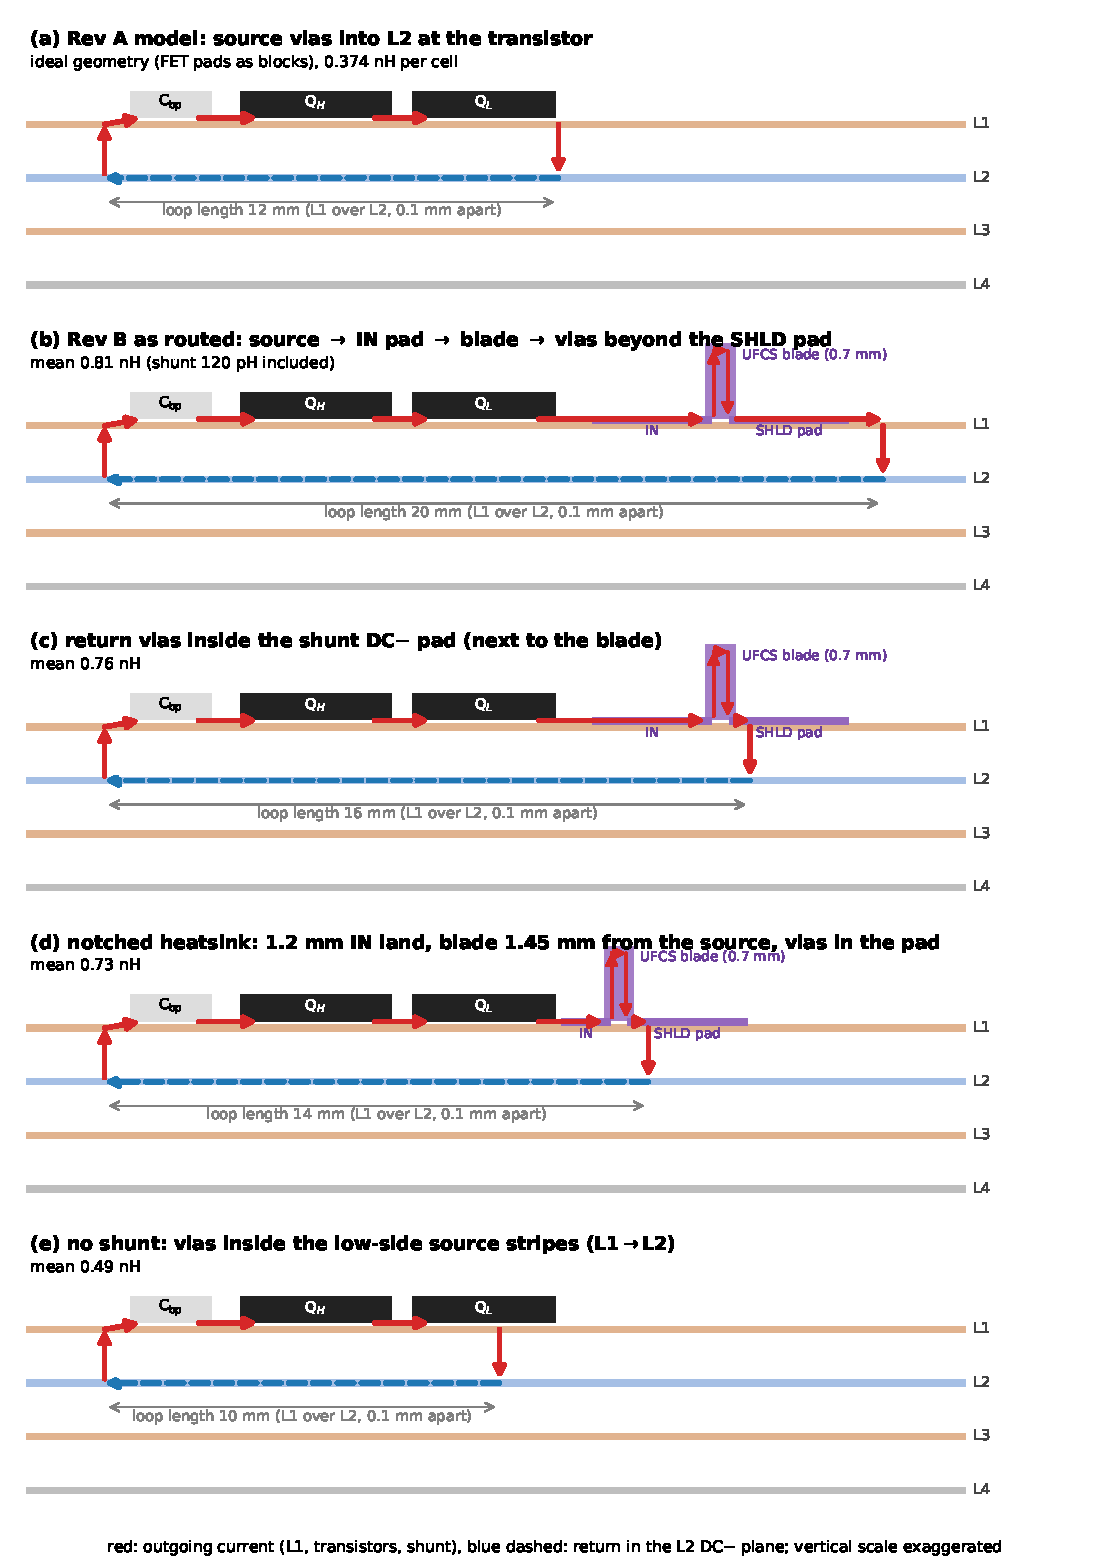
\includegraphics[width=0.95\linewidth]{figs/loop_paths.pdf}
\caption{Loop current paths (exploded side view along one cell, vertical scale exaggerated). The UFCS is a thin blade
soldered upright across the gap between its IN and SHLD pads: the current crosses only at the blade.}
\end{figure}

\paragraph{1. The \SI{0.374}{nH} was a geometry-model value.} It came from the idealised building-block geometry in which
the transistor pads are solid blocks and full via rows sit next to them. On the routed board the EPC2361 pads are
interleaved drain/source stripes: a via row under the transistor cuts stripes of the other net and was removed by the
clearance check (switch-node row 1--2 of about 10 vias per cell, source row 0--2 of about 10). Without the shunt and with
vias placed \emph{inside} the source stripes (L1$\rightarrow$L2 blind vias, the method recommended for GaN
packages), the routed Rev B cell reaches \Lnoshunt\,nH on average (0.42\,nH in cells 2/4).

\paragraph{2. The shunt path.} The UFCS blade is \SI{0.7}{mm} thick and \SI{15}{mm} wide (across the cell); the
recommended footprint is two \SI{15}{mm}\,$\times$\,\SI{3}{mm} pads. The current must reach the blade, i.e.\ cross the 3\,mm IN pad, and
return from the SHLD side into L2. As routed the return vias sit below the SHLD pad, about \SI{4}{mm} past the blade.
Shunt as routed versus no shunt: \Lbase\ versus \Lnoshunt\,nH, i.e.\ about 0.12\,nH for the shunt itself plus about 0.2\,nH of copper
detour.

\paragraph{3. Left/right asymmetry.} Cells 1 and 3 (left cell of each pair) are about 0.14\,nH above cells 2 and 4 in
every variant, also without the shunt: the left transistors are rotated by \SI{180}{\degree} (not mirrored), so the
stripe/via arrangement under the left and right cell differs. This must be corrected in the cell layout.

\section{Results}
\begin{figure}[H]
\centering
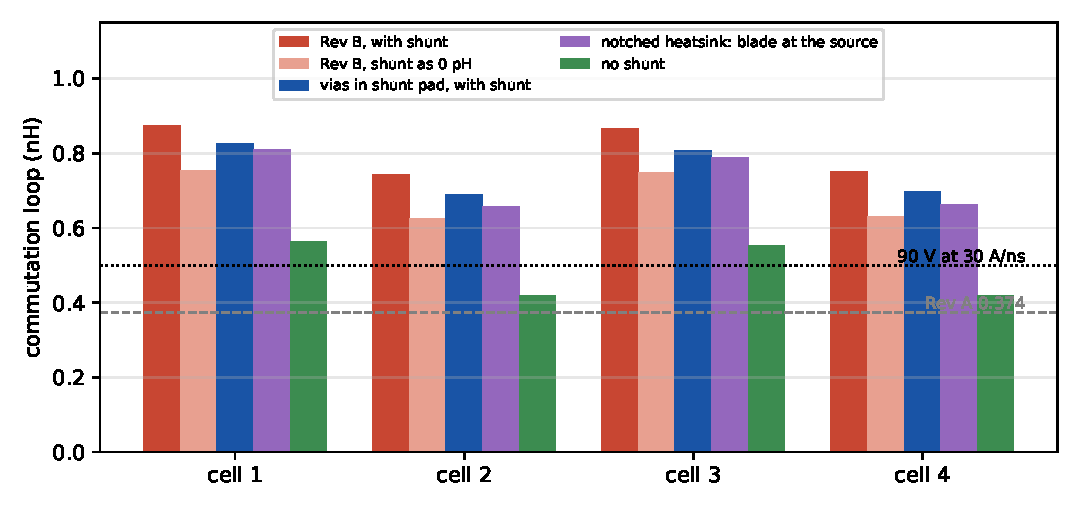
\includegraphics[width=0.9\linewidth]{figs/loop_per_cell.pdf}
\caption{Commutation loop per cell, all four low-side FETs switching.}
\end{figure}

\begin{table}[H]
\centering\small
\begin{tabular}{@{}lrrrrrrr@{}}
\toprule
Variant & cell 1 & cell 2 & cell 3 & cell 4 & mean & $\hat v_\mathrm{DS}$ (V) & $di/dt$ for \\
 & \multicolumn{5}{c}{nH} & at 30\,A/ns & 90\,V (A/ns) \\
\midrule
Rev B as routed (UFCS 120\,pH) & 0.875 & 0.744 & 0.867 & 0.751 & 0.809 & 99 & 19 \\
Rev B, shunt replaced by 0\,pH & 0.755 & 0.624 & 0.747 & 0.631 & 0.689 & 96 & 22 \\
Rev B, without the bottom bypass row & 0.895 & 0.763 & 0.888 & 0.770 & 0.829 & 100 & 18 \\
Return vias in the shunt DC$-$ pad (UFCS 120\,pH) & 0.826 & 0.691 & 0.807 & 0.698 & 0.755 & 98 & 20 \\
Return vias in the pad, shunt 0\,pH & 0.706 & 0.571 & 0.688 & 0.578 & 0.635 & 94 & 24 \\
Blade 1.45\,mm from the source + vias in pad (notch) & 0.809 & 0.658 & 0.788 & 0.663 & 0.729 & 97 & 21 \\
No shunt, source vias to L2 & 0.563 & 0.420 & 0.552 & 0.420 & 0.488 & 90 & 31 \\
\midrule
Rev A geometry model & \multicolumn{4}{c}{0.374} & 0.374 & 86 & 40 \\
\bottomrule
\end{tabular}

\caption{Loop per cell; $\hat v_\mathrm{DS} = 75\,\mathrm{V} + L\,di/dt$.}
\end{table}

\begin{itemize}
\item \textbf{Return vias inside the SHLD pad} (filled and capped via-in-pad): \Lvip\,nH, the return starts next to the
blade instead of \SI{4}{mm} below it.
\item \textbf{Blade at the source (notched heatsink)}: IN land shortened to \SI{1.2}{mm} (solder fillet; the manual allows
soldering across a short cut, p.\,12), blade \SI{1.45}{mm} from the source copper, vias in the SHLD pad: \Lnotch\,nH
(\Vnotch\,V at 30\,A/ns, $\le$\,90\,V up to \Dinotch\,A/ns).
\item \textbf{Bottom bypass row}: \Ltoponly\,nH; it serves the charge hand-over to the bank, not the loop.
\end{itemize}

\section{Mechanical constraint: the heatsink}
The blade position is not set by the electrical layout but by the heatsink: the UFCS body above the blade is
\SI{7.5}{mm} thick (\SI{\pm3.75}{mm} around the blade) and \SI{27}{mm} tall, the top-side heatsink (LAM\,4 on the
spreader) covers the transistors and ends at $y = \SI{11.3}{mm}$; with the blade at \SI{15.25}{mm} the body starts at
\SI{11.5}{mm}. In the notch variant the body overhangs the low-side FET by about \SI{2}{mm} at \SI{4.1}{mm} height:
the spreader must be stepped there ($\le$\,\SI{3.2}{mm} above the FET) and the heatsink edge moved to $y\approx\SI{8.8}{mm}$
at the shunts. The shortened IN land is \SI{0.2}{mm} from the low-side FET pads, so the courtyards overlap: the blade
has to be soldered by hand after the FETs (as the manual recommends anyway).

\section{Conclusions}
\begin{enumerate}
\item Most of the difference to the \SI{0.374}{nH} model is the routed cell itself (vias removed by the stripes);
vias inside the source stripes are needed in any case. Without the shunt the routed cell reaches \Lnoshunt\,nH.
\item The shunt path costs about 0.3\,nH as routed; return vias in the SHLD pad and the blade at the source reduce it to the
values above.
\item The left/right difference of about 0.14\,nH between the cells of a pair is a layout asymmetry (rotated, not
mirrored transistors) and has to be removed before the next release.
\item With the shunt fitted the overshoot limit of 90\,V needs $di/dt \le$\,\Dinotch\,A/ns even in the best variant;
for the load test a shunt-free assembly (copper link, source vias) gives \Dinoshunt\,A/ns.
\end{enumerate}
\end{document}
